\section*{Problema 3}

\textbf{Implemente el algorito de cuadratura de Gauss-Legendre y evalua las integrales usando 2, 4 y 10 nodos.}

\begin{enumerate}
    \item \begin{equation*}
              \int_0^\pi xcos(x) dx
          \end{equation*}

          \begin{figure}[H]
            \centering
            \begin{subfigure}[b]{8cm}
                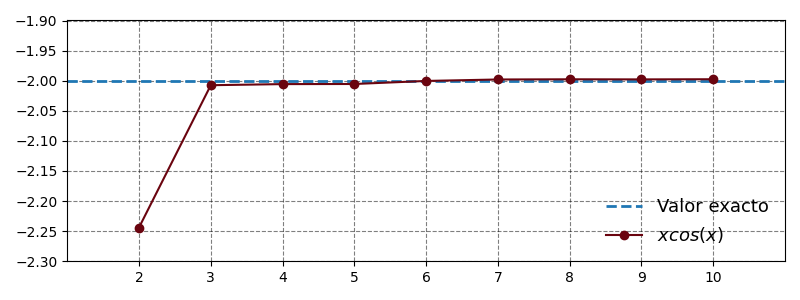
\includegraphics[width=8cm]{Graphics/problema03_fun_f1.png}
                \caption{}
            \end{subfigure}
            \begin{subfigure}[b]{8cm}
                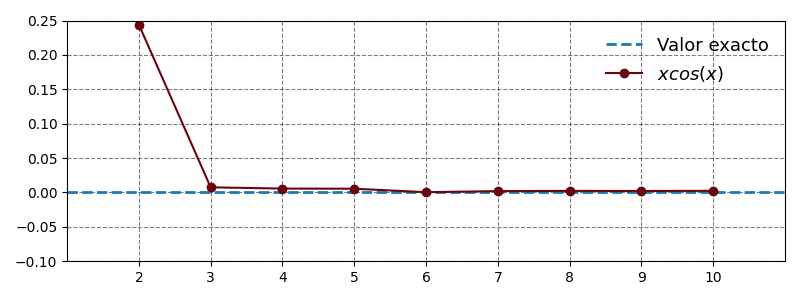
\includegraphics[width=8cm]{Graphics/problema03_diff_f1.png}
                \caption{}
            \end{subfigure}
            \caption{}
        \end{figure}

    \item \begin{equation*}
              \int_{-1}^0 xe^{-x} dx
          \end{equation*}

          \begin{figure}[H]
            \centering
            \begin{subfigure}[b]{8cm}
                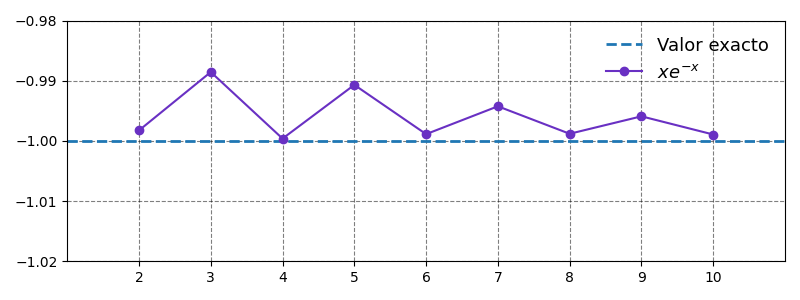
\includegraphics[width=8cm]{Graphics/problema03_fun_f2.png}
                \caption{}
            \end{subfigure}
            \begin{subfigure}[b]{8cm}
                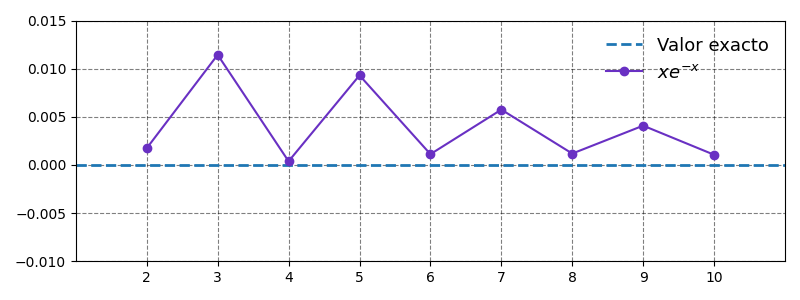
\includegraphics[width=8cm]{Graphics/problema03_diff_f2.png}
                \caption{}
            \end{subfigure}
            \caption{}
        \end{figure}
\end{enumerate}